\documentclass[11pt]{article}
\usepackage[T1]{fontenc}
\usepackage{lmodern}
\usepackage[margin=1.05in]{geometry}
\usepackage{amsmath,amssymb,amsthm,mathtools}
\usepackage{mathrsfs}
\usepackage{microtype}
\input{glyphtounicode-cmex}
\pdfgentounicode=1
\usepackage{etoolbox}
\usepackage{enumitem}
\usepackage{booktabs,array}
\usepackage{tikz}
\usetikzlibrary{arrows.meta,positioning,calc,decorations.pathreplacing}
\usepackage[numbers,sort&compress]{natbib}
\usepackage[colorlinks=true,linkcolor=blue!55!black,citecolor=blue!55!black,urlcolor=blue!55!black]{hyperref}
\usepackage[nameinlink,capitalise,noabbrev]{cleveref}
\makeatletter
\def\CharacterThmRefstepcounter{%
  \@ifnextchar[{\CharacterThmRefstepcounterOpt}%
    {\Hy@theorem@refstepcounter}}
\def\CharacterThmRefstepcounterOpt[#1]#2{%
  \let\CharacterSavedRefstepcounter\cref@old@refstepcounter
  \let\cref@old@refstepcounter\Hy@theorem@refstepcounter
  \refstepcounter@optarg[#1]{#2}%
  \let\cref@old@refstepcounter\CharacterSavedRefstepcounter}
\patchcmd{\cref@thmnoarg}
  {\refstepcounter}{\CharacterThmRefstepcounter}
  {}{\PackageError{character-varieties}{Theorem anchor patch failed}{}}
\patchcmd{\cref@thmoptarg}
  {\refstepcounter}{\CharacterThmRefstepcounter}
  {}{\PackageError{character-varieties}{Typed theorem anchor patch failed}{}}
\makeatother
\AddToHook{cmd/thebibliography/after}{\addcontentsline{toc}{section}{\refname}}
\newtheorem{theorem}{Theorem}[section]
\newtheorem{proposition}[theorem]{Proposition}
\newtheorem{lemma}[theorem]{Lemma}
\newtheorem{corollary}[theorem]{Corollary}
\theoremstyle{definition}
\newtheorem{definition}[theorem]{Definition}
\newtheorem{remark}[theorem]{Remark}
\newtheorem{example}[theorem]{Example}
\newcommand{\C}{\mathbb C}
\newcommand{\Q}{\mathbb Q}
\newcommand{\Z}{\mathbb Z}
\newcommand{\A}{\mathbb A}
\newcommand{\Gm}{\mathbb G_m}
\newcommand{\cO}{\mathcal O}
\DeclareMathOperator{\GL}{GL}
\DeclareMathOperator{\SL}{SL}
\DeclareMathOperator{\Spec}{Spec}
\DeclareMathOperator{\Hom}{Hom}
\DeclareMathOperator{\End}{End}
\DeclareMathOperator{\rk}{rk}
\DeclareMathOperator{\tr}{tr}
\DeclareMathOperator{\Ad}{Ad}
\DeclareMathOperator{\Irr}{Irr}
\DeclareMathOperator{\diag}{diag}
\DeclareMathOperator{\im}{im}
\DeclareMathOperator{\ord}{ord}
\setlist{itemsep=2pt,topsep=5pt}
\setlength{\emergencystretch}{2em}
\title{Integral points on character varieties of curves}
\author{OpenAI}
\date{September 25, 2026}
\hypersetup{pdftitle={Integral points on character varieties of curves},pdfauthor={OpenAI}}
\pdfinfoomitdate=1
\pdftrailerid{}
\pdfsuppressptexinfo=15
\begin{document}
\maketitle
\begin{abstract}
We prove potential Zariski density of integral points on $\SL_r$-character
varieties of smooth complex curves in every rank. The result allows
prescribed quasi-unipotent boundary monodromy, including exact nonsemisimple
conjugacy classes, and holds on every component over the full ring of
integers of one finite extension. Here integrality is measured in the
ambient character variety, while the exact boundary conditions are imposed
on the complex representation.
\end{abstract}
\tableofcontents
\section{Introduction}\label{sec:introduction}

Let $X$ be a smooth connected complex algebraic curve and let $r\geq1$.
Its $\SL_r$-character variety parametrizes semisimple representations of
$\pi_1(X)$ up to isomorphism. Although $X$ need not be defined over a number
field, this character variety has a natural integral model: a finite
presentation of its fundamental group gives a representation scheme over
$\Z$, and we take the spectrum of its ring of conjugation invariants.
Write this affine scheme as $M_r(X)$.

An arithmetic question is whether its integral points become Zariski dense
after extending the ground field once. Here integrality always refers to
the full ring of integers. We prove this for curves, retaining arbitrary
quasi-unipotent conjugacy classes at the punctures.

Let $\overline X$ be the smooth projective completion of $X$, and write
$\overline X\setminus X=\{x_1,\ldots,x_s\}$. For each $i$, fix a positive
meridian $\gamma_i$ about $x_i$. A matrix is \emph{quasi-unipotent} if all
its eigenvalues are roots of unity. Choose quasi-unipotent conjugacy
classes $C_i\subset\SL_r(\C)$, and let $Y$ be the reduced locus in
$M_r(X)_\C$ whose semisimple representations have
$\rho(\gamma_i)\in C_i$. This condition allows nonsemisimple boundary
matrices: semisimplicity of a representation is a condition on the whole
group action. The locus $Y$ is locally closed, as explained in
Section~\ref{sec:model}.

For a number field $L\subset\C$, write $\cO_L$ for its full ring
of integers.  We use \emph{ambient} integrality on $Y$: a point
extends to $M_r(X)$ over $\cO_L$, and its complex semisimple
representation has the specified boundary classes.  It need not
avoid smaller Jordan classes after reduction at every finite prime.
Requiring a section of a strict locally closed integral model is
a different condition.

\begin{theorem}\label{thm:main}
Let $X$ be a smooth connected complex algebraic curve and let $r\geq1$.
For prescribed quasi-unipotent conjugacy classes $C_1,\ldots,C_s$ as above,
let $K\subset\C$ be a number field containing their eigenvalues. There is
a finite extension $L/K$ such that
\[
 M_r(X)(\cO_L)\cap Y(\C)
\]
is Zariski dense in $Y$, and hence in every irreducible component of $Y$.
The same conclusion holds when only the characteristic polynomial of
each boundary monodromy is prescribed, with all its roots roots of unity.
It also holds for the entire character variety without boundary
conditions; in that case one may take $K=\Q$.

For the relative statements and for projective $X$, one may take distinct
primes $p,q>r$ and
\begin{equation}\label{eq:main-field}
 F=K(\sqrt2,\zeta_{pq}),\qquad
 L=F\bigl(\zeta_r,\{u^{1/r}:u\in\cO_F^\times\}\bigr),
\end{equation}
where $\zeta_m$ denotes a primitive $m$th root of unity. In the projective
case there are no boundary conditions and $K=\Q$.
\end{theorem}

The extension in \eqref{eq:main-field} is finite because the unit group
of $\cO_F$ is finitely generated. It is fixed for the entire locus,
including all its components. No restriction on the genus or on the
Jordan forms is imposed.

For a nonprojective curve without boundary conditions, density already
holds over $\Z$: the fundamental group is free and $\SL_r(\Z)$ is
Zariski dense in $\SL_r(\C)$. The substantive cases here are prescribed
boundary monodromy and projective curves, where the surface relation
couples the matrices. We construct actual integral representations and
then pass to their characters; the exact boundary conditions are selected
only after this passage.

\subsection{History and relation to previous work}

The arithmetic study of local systems includes Simpson's conjecture
that rigid irreducible representations of smooth projective fundamental
groups are defined over rings of integers~\cite[p.~9]{Simpson1992}.
Esnault and Groechenig prove integrality for irreducible cohomologically
rigid local systems with finite determinant and quasi-unipotent boundary
monodromy on smooth quasiprojective varieties~\cite[Theorem~1.1]{EsnaultGroechenig2018}.
Here an integral local system may have a finite projective lattice over a
number ring; freeness is not part of that assertion.
Without a rigidity assumption, de Jong and Esnault prove that the
existence of an irreducible complex local system with torsion determinant
and quasi-unipotent boundary monodromy implies the existence of an
absolutely irreducible integral $\ell$-adic local system for every prime
$\ell$, preserving the determinant and the semisimplified boundary
classes~\cite[Theorem~1.1]{DeJongEsnault2024}.
This prime-by-prime existence is distinct from density over the full ring
of integers of one number field.

Litt asks for potential integral density on character varieties of smooth
projective varieties and also formulates a boundary
variant~\cite{LittProblems}; his survey explicitly asks whether one
number field suffices~\cite[Question~5.4.3(2)]{Litt2024}.
Coccia and Litt formulate a related
conjecture for Chevalley groups with fixed boundary data in the adjoint
quotient~\cite[Conjecture~1.1.1]{CocciaLitt}. Theorem~\ref{thm:main}
answers the determinant-one form of Litt's question affirmatively for
curves, in every rank, and proves the $\SL_r$ curve case of the
Coccia--Litt conjecture for quasi-unipotent boundary data.
The higher-dimensional, higher-rank question remains outside its scope.

Coccia and Litt prove full-ring potential integral density for $\SL_2$
and $\mathrm{PGL}_2$ on smooth varieties admitting a smooth projective
compactification with simple normal crossings boundary~\cite[Theorem~1.1.2]{CocciaLitt}.
Their surface theorem allows arbitrary algebraic-integer boundary traces
and gives an extension of degree at most four over the field generated
by those traces~\cite[Theorem~5.0.4 and Remark~5.0.5]{CocciaLitt}.
Their ordinary and twisted surface theorems also imply the ambient-integral
exact-class statement in rank two, as explained in
Remark~\ref{rem:rank-two-comparison}.
Their use of integral representations and mapping-class-group dynamics
is an arithmetic predecessor of the closed-surface argument below.
Theorem~\ref{thm:main} treats every rank with exact quasi-unipotent
boundary data; in rank two, Coccia and Litt allow a broader range of
boundary traces.

Earlier arithmetic work includes Whang's descent framework for
rank-two integral characters with fixed integer boundary
traces~\cite{WhangDescent}. For the Markoff cubic family
$x^2+y^2+z^2-xyz=k$, Ghosh and Sarnak prove integral density for
almost all locally admissible integer parameters, and also exhibit
infinitely many admissible parameters with no integral
points~\cite[Theorem~1.2]{GhoshSarnak}. These results concern ordinary
integral points and help distinguish that question from density
after one finite extension of the ground field.

On the geometric side, Mellit uses flags and braid operations to stratify
a vector bundle over a character variety into torus and affine-space
pieces, for generic semisimple data with a regular semisimple
puncture~\cite[Theorem~1.2]{Mellit}. Su constructs an open dense torus
for nonempty character varieties with generic semisimple boundary data
and a regular semisimple puncture~\cite[Theorem~0.5]{Su}.
These results concern complex geometric decompositions. The present
argument must also preserve integral splittings and identified graded
modules while treating arbitrary Jordan types and nongeneric components.
It therefore carries out the local operations over the full ring of
integers, rather than obtaining integral points merely from a complex
coordinate parametrization.

\subsection{The proof}

We first work with $\GL_n$ rather than $\SL_n$. This makes direct sums,
subspaces and quotients available without determinant restrictions.
A boundary matrix with a prescribed Jordan type admits an invariant
flag on whose successive quotients it acts by scalar roots of unity.
We attach disks carrying these scalar local systems to the boundary.
The resulting object consists of oriented surfaces of various ranks,
joined along boundary pieces by flags and their graded identifications.
Section~\ref{sec:diagrams} defines exactly which joins are allowed.

The main construction proves integral density for all such diagrams by
induction on the largest rank. A surface of maximal rank with boundary
is cut into disks. Two flags at the ends of a cut are compared by
refining them to their common graded pieces and interchanging adjacent
pieces. On each disk, a proper subspace chosen from one boundary flag
is preserved by all puncture monodromies, since these are scalar. Passing
to that subspace and its quotient lowers the rank. The lost extension
data are recovered by successive choices of linear maps. Choosing the
subspace as a prefix of the starting flag makes the lifted flag unique
on that interval, so returning around the boundary introduces no further
equation.
The reduction includes the complementary swaps needed for
nonregular boundary data (Section~\ref{sec:reduction}).

Closed surfaces enter at the same induction step. Cutting along one
nonseparating circle and fixing a convenient spectrum brings them into
the preceding case. Powers of a Dehn twist then enlarge the closure of
the integral points. At one explicit smooth representation, the
resulting torus motions vary the spectrum in every direction.
Irreducibility of the twisted surface equation finishes the argument.
We give a finite-field proof of irreducibility, following the
character-counting method of Liebeck and Shalev~\cite{LiebeckShalev2005}.
Sections~\ref{sec:surfaces} and~\ref{sec:dynamics} carry out this
closed-surface step; the latter then assembles the rank induction.

Finally, all handle determinants of our integral representations are
units in $\cO_F$. Adjoining their $r$th roots uniformly by
\eqref{eq:main-field} permits determinant-one twisting. Exact Jordan
conditions are then selected on the character quotient. This order is
essential: taking the semisimplification of a representation can reduce
its boundary Jordan blocks. Section~\ref{sec:descent} completes this descent.

The reusable ingredient is the diagram density theorem. It transfers
integral density through rank reduction using free graded modules and
linear extension parameters.

Three standard inputs enter at distinct points.  Finite generation
of integral invariants gives the affine model in
Section~\ref{sec:model}.  Dirichlet's unit theorem gives the single
field in Section~\ref{sec:arithmetic}.  The Lang--Weil estimate
converts the finite-group count proved in Section~\ref{sec:surfaces}
into geometric irreducibility.  The flag reconstruction, character
estimates, twist directions and exact-Jordan descent are proved below.

\section{The integral model and exact boundary conditions}\label{sec:model}

We specify the integral model once and record how to select exact
boundary classes on its complex quotient. In particular, we distinguish
semisimplification of a representation from diagonalization of its
individual matrices.

\subsection{Representation schemes}

For a finitely presented group $\Gamma$ and an integer $r\geq1$, let
$\mathscr R_r(\Gamma)$ be the affine $\Z$-scheme representing
\[
 S\longmapsto\Hom(\Gamma,\SL_r(S)).
\]
Concretely, choose a matrix for each generator and impose the matrix
relations of a finite presentation. Simultaneous conjugation defines
an action of $\SL_{r,\Z}$. With
$A=\Z[\mathscr R_r(\Gamma)]$, put
\begin{equation}\label{eq:integral-model}
 M_r(\Gamma)=\Spec\bigl(A^{\SL_{r,\Z}}\bigr).
\end{equation}
This definition is independent of the chosen presentation, by the
representing property. The invariant ring is finitely generated over
$\Z$ by finite generation for Chevalley-group invariants
\cite[Theorem~3]{FranjouVanderKallen}.
Here the base $\Z$ is Noetherian, $A$ is a finite-type commutative
algebra, and $\SL_{r,\Z}$ is a split Chevalley group with its
rational conjugation action.  This input does not require $A$ to
be reduced or flat over $\Z$.

Flat base change commutes with these invariants: they are the kernel of
the difference between the coaction and the map $a\mapsto a\otimes1$,
and tensoring with a flat algebra preserves that kernel. In particular,
the complex fiber of \eqref{eq:integral-model} is the usual affine
character quotient. Its complex points correspond to the unique closed orbits
in the fibers of the quotient~\cite[pp.~184--185]{MumfordSuominen}.
The representation scheme is closed in the space of generator
tuples: inverses in $\SL_r$ are polynomial adjugates, so the
relators are polynomial equations. Kraft's matrix-tuple closed-orbit
criterion, recalled in \cite[Section~3.4]{BateMartinRoehrleTange},
therefore identifies these orbits with semisimple representations.
Conjugation by $\GL_r(\C)$ gives the same orbits as conjugation by
$\SL_r(\C)$, since any invertible matrix can be multiplied by a scalar
to have determinant one.

For the curve $X$, we use $\Gamma=\pi_1(X)$ and write $M_r(X)=M_r(\Gamma)$.
Every representation $\Gamma\to\SL_r(\cO_L)$ gives a point of
$M_r(X)(\cO_L)$ by evaluating invariant functions. Thus it suffices to
construct actual integral matrices. No assertion about generation of
invariants in positive characteristic is needed for this implication.

\subsection{Rank conditions on the quotient}

Write $\mathscr R=\mathscr R_r(\Gamma)_\C$ and let
$q:\mathscr R\to M_r(\Gamma)_\C$ be the quotient map. We use reduced
closed subsets when imposing additional conditions. An invariant closed
subset $D\subset\mathscr R$ has closed image under $q$. Moreover,
\begin{equation}\label{eq:closed-orbit-test}
 q(x)\in q(D)
 \quad\Longleftrightarrow\quad
 \text{the closed orbit in }q^{-1}(q(x))\text{ lies in }D.
\end{equation}
Indeed the closure of every orbit in the fiber contains that closed
orbit, and a closed invariant subset contains the closure of each of
its orbits. These are the standard closed-orbit properties of an affine
quotient by a reductive group in characteristic zero~\cite[pp.~184--185]{MumfordSuominen}.

Fix the characteristic polynomial of each boundary matrix and let
$\lambda$ range over its eigenvalues. A Jordan form is determined by
these eigenvalues and the numbers
\[
 d_{i,\lambda,k}=\rk\bigl((C_i-\lambda I)^k\bigr),
 \qquad 1\leq k\leq r.
\]
Here the expression on the right means the rank for any matrix in
the chosen class $C_i$. Let $D$ be the invariant closed subset defined
by the fixed characteristic polynomials and the inequalities
\[
 \rk\bigl((\rho(\gamma_i)-\lambda I)^k\bigr)
 \leq d_{i,\lambda,k}.
\]
Let $D_{\mathrm{sm}}\subset D$ be the finite union of the closed subsets
on which at least one of these inequalities is strict; indices with
$d_{i,\lambda,k}=0$ contribute an empty subset. The matrices have exactly
the prescribed classes precisely on $D\setminus D_{\mathrm{sm}}$.

\begin{lemma}\label{lem:exact-stratum}
The locus of characters whose semisimple representations have exactly
the prescribed boundary classes is
\[
 Y=q(D)\setminus q(D_{\mathrm{sm}}).
\]
In particular, $Y$ is open in the closed subset $q(D)$ and is defined
over any number field containing the boundary eigenvalues.
\end{lemma}

\begin{proof}
Apply \eqref{eq:closed-orbit-test} first to $D$, then to
$D_{\mathrm{sm}}$. A closed orbit belongs to the first set and not the
second exactly when its boundary matrices have all the prescribed
ranks. These ranks determine their Jordan forms. The defining
equations and rank inequalities have coefficients in the indicated
field $K$.  Write $A_K=A\otimes_{\Z}K$.  If $I_K\subset A_K$ is
the ideal of either closed rank locus, its closed quotient image is defined by the
contracted ideal $I_K\cap A_K^{\SL_r}$.  This is the kernel of
$A_K^{\SL_r}\to A_K/I_K$; flat extension from $K$ to $\C$ preserves
that kernel and the invariant algebra.  The two closed images, and
hence their difference, are therefore defined over $K$.
\end{proof}

The lemma permits us to construct integral representations in closed
rank bounds and impose the exact conditions after passing to characters.
Density will then meet every open part of the desired locus, including
those in individual irreducible components.

\section{Arithmetic parameters and integral splittings}
\label{sec:arithmetic}

Our constructions will use matrices, split flags, and gluing maps over one
ring of integers.  We first record the parameter sets that are dense over
that ring and the finite extension needed to remove determinants.

Fix the rank bound $r\geq 1$ and a number field $K\subset\C$ containing
the prescribed boundary eigenvalues.  Choose distinct primes $p,q>r$,
fix a primitive $pq$-th root of unity $\zeta$, and put
\[
 F=K(\sqrt{2},\zeta),\qquad R=\cO_F.
\]
For a projective curve we take $K=\mathbb Q$.  Throughout the proof,
``integral'' means over the full ring $R$, or over the full ring of
integers of a specified finite extension.  In particular, an invertible
integral matrix belongs to $\GL_d(R)$: its determinant is a unit.

\begin{lemma}\label{lem:integral-parameters}
For every $a,b\geq 0$, the set
$R^a\times(R^\times)^b$ is Zariski dense in
$\C^a\times(\C^\times)^b$.  For every $d\geq 1$, the group
$\GL_d(R)$ is Zariski dense in $\GL_d(\C)$.
\end{lemma}

\begin{proof}
The sets $R$ and $R^\times$ are infinite.  For the unit group,
use the powers of the unit $1+\sqrt{2}$, whose inverse is
$\sqrt{2}-1$.  A polynomial vanishing on a product of infinite subsets
of $\C$ is zero, by induction on the number of variables.  Multiplying
a Laurent polynomial by a monomial gives the same conclusion for the
stated product with multiplicative factors.

For $d\geq 2$, the Zariski closure of $\GL_d(R)$ contains every elementary
one-parameter unipotent subgroup, since its parameters in $R$ are dense.
These subgroups generate $\SL_d(\C)$.  The closure also contains the full
diagonal torus, by the first assertion.  Together these generate
$\GL_d(\C)$.  The case $d=1$ is unit density.
\end{proof}

We will always supply free graded modules as part of integral flag data.
This requirement permits the following elementary splitting argument over
$R$, without any assumption on its ideal class group.

\begin{lemma}\label{lem:free-splittings}
Let $0\to A\to B\to C\to 0$ be an exact sequence of $R$-modules, with
$A$ and $C$ finite free.  Then the sequence splits over $R$.  Its sections
form a nonempty affine space under $\Hom_R(C,A)$, and their integral
points are Zariski dense in the complex space of sections.
Consequently, a finite filtration with specified free graded modules
admits a splitting over $R$ that respects those graded identifications.
\end{lemma}

\begin{proof}
Lift an $R$-basis of $C$ to $B$ and extend linearly to obtain a section.
The difference of any two sections is an arbitrary map from $C$ to $A$.
After choosing bases this is a free matrix module, so density follows
from Lemma~\ref{lem:integral-parameters}.  Apply the splitting argument
successively to the quotients of a filtration.
\end{proof}

In particular, every matrix changing between two such integral splittings
is an $R$-isomorphism; its inverse is integral.  This argument concerns
flags whose graded modules are explicitly free.  We will establish that
property for each flag used below.

\begin{lemma}\label{lem:unit-spectrum}
For every $1\leq n\leq r$, the units
\[
 \alpha_i=\zeta^{i-1},\qquad 1\leq i\leq n,
\]
are distinct, and $\alpha_i-\alpha_j\in R^\times$ whenever $i\ne j$.
\end{lemma}

\begin{proof}
The nonzero integer $i-j$ has absolute value less than both $p$ and $q$,
so it is prime to $pq$.  Thus $\zeta^{i-j}$ is primitive of order $pq$.
The algebraic integer $1-\zeta^{i-j}$ has norm
$\Phi_{pq}(1)=1$ in $\mathbb Q(\zeta)$, and hence is a unit.  Here the
value follows directly by taking $T\to1$ in
\[
 \Phi_{pq}(T)=
 \frac{(T^{pq}-1)(T-1)}{(T^p-1)(T^q-1)}.
\]
Multiplication by the unit $\zeta^{j-1}$ proves the claim.
\end{proof}

The unit differences in Lemma~\ref{lem:unit-spectrum} allow spectral
projectors to be formed over $R$.  The freeness of their images, when
needed, will follow from the free graded lines of the accompanying flag.

\begin{lemma}\label{lem:uniform-field}
The field
\[
 L=F\bigl(\zeta_r,\{u^{1/r}:u\in R^\times\}\bigr)
\]
is a finite extension of $F$.  It contains every $r$-th root of every
unit of $R$, and every such root belongs to $\cO_L^\times$.
\end{lemma}

\begin{proof}
By Dirichlet's unit theorem~\cite[Theorem~5.1]{MilneANT}, choose finitely
many generators
$u_0,\ldots,u_s$ of $R^\times$, including a generator of its finite
torsion subgroup.  Choose $v_i$ with $v_i^r=u_i$.  The finite extension
\[
 F(\zeta_r,v_0,\ldots,v_s)
\]
contains all $r$-th roots of all units: if
$u=\prod_i u_i^{m_i}$ with $m_i\in\Z$, its roots are
$\zeta_r^j\prod_i v_i^{m_i}$.
Both $v_i$ and $v_i^{-1}$ are integral, by the monic equations
$T^r-u_i$ and $T^r-u_i^{-1}$, respectively.  Hence all these roots are
units in $\cO_L$.
\end{proof}

The field $L$ depends only on the fixed initial data.  Later we will take
roots of determinants of matrices over $R$; Lemma~\ref{lem:uniform-field}
handles all those roots simultaneously, regardless of the representation
or irreducible component.

\section{Filtered local systems on surfaces}
\label{sec:diagrams}

The proof uses auxiliary surfaces whose boundary local systems are related
by filtrations.  Cutting these surfaces and refining their filtrations
will reduce the rank.  We first define the auxiliary objects and the
linear algebra needed to reconstruct them after a cut.

Use the field $F$ and its full ring of integers $R$ from
Section~\ref{sec:arithmetic}.  All prescribed
scalars below are roots of unity in $F$.  A local system over $R$ is
required to have finite free fibers.  Its parallel transports are thus
isomorphisms over the full ring $R$.

\subsection{Surfaces, seams, and their solutions}

A \emph{surface diagram} has finitely many compact oriented surfaces,
called its facets.  Each facet has an assigned rank between $0$ and $r$
and finitely many interior punctures.  A scalar monodromy is prescribed
at each puncture, using the positive orientation around that puncture.

Every boundary circle is either left unmarked or divided into intervals
by finitely many marked points.  These boundary pieces are grouped into
\emph{seams}.  A seam has a distinguished parent side and an ordered
list of child sides, written
\[
 E:(W_1,\ldots,W_m),\qquad
 \rk E=\sum_{j=1}^m\rk W_j.
\]
All its sides are parametrized by the same interval or circle.  The
boundary orientation of each child is opposite to that of the parent.
Different side occurrences may belong to the same facet.  An unmarked
circle seam uses entire circles and has no permutation of its sides.

At an interval endpoint, the boundary of each facet pairs its two
incident side germs.  We permit precisely the following vertices.
\begin{enumerate}
\item A parent list continues with the same ordered children, or with
two adjacent children interchanged.  Each child continues to itself.
\item A child $W$ of one parent list is replaced by an ordered list
$W'_1,\ldots,W'_s$, and there is a third seam
$W:(W'_1,\ldots,W'_s)$.  The parent germs continue to each other;
the two occurrences of $W$ are paired; the two occurrences of each
$W'_j$ are paired; and unchanged children continue to themselves.
The reverse operation is also permitted.
\end{enumerate}
The specification concerns distinct occurrences of germs, even when
some belong to one facet.  No embedding of the diagram in a surrounding
space is required.

A \emph{solution} assigns to each punctured facet a local system of its
rank, with the prescribed scalar monodromies.  At a seam it assigns a
parallel filtration of the parent and parallel identified quotients
\[
 0=E_0\subset E_1\subset\cdots\subset E_m=E,
 \qquad E_j/E_{j-1}\simeq W_j.
\]
The conditions at vertices are as follows.  At a continuation, all data
continue.  At a split or merge, the finer parent filtration is obtained
by refining the $W$-quotient with its given filtration, and the
identified quotients agree.  At an interchange of $A,B$, the coarsened
filtration with quotient $A\oplus B$ is unchanged.  Within that quotient
the two intermediate subspaces are complementary, and the maps to
the identified quotients are the natural projections.  Thus the
interchange includes a specified direct-sum decomposition, not just a
pair of transverse flags.

Choose one frame on each connected facet.  Holonomies along a finite
set of paths, the seam flags, and their identified quotients describe
the solutions by finitely many algebraic equations and open conditions.
They form a complex variety, denoted $\mathcal S(D)$ for a diagram $D$.
Changing the auxiliary paths gives the same data through composition
and inversion of transport matrices.

An \emph{integral solution} uses free $R$-local systems and filtrations
whose identified graded modules are the specified free child fibers.
Complementarity at an interchange means a direct sum over $R$.
In particular, each filtration splits on a fiber: successive free
quotients are projective.  This definition does not assert that every
submodule of a free $R$-module is free.

\begin{theorem}[Diagram density]\label{thm:diagram-density}
For every surface diagram $D$ with ranks at most $r$ and prescribed
scalar puncture monodromies in $F$, its integral solutions over $R$
are Zariski dense in $\mathcal S(D)$.
\end{theorem}

We prove Theorem~\ref{thm:diagram-density} by induction on the largest
rank, normalizing identity seams before separating closed facets.
The nonclosed step is proved in Section~\ref{sec:reduction}.
The rank-one and genus-zero closed cases are elementary, and the
genus-one case is Lemma~\ref{lem:torus-density}.  At each remaining
rank, Lemma~\ref{lem:closed-density} gives the closed-surface step;
it uses the normalized nonclosed step at that same rank and the
completed induction at smaller ranks.

\subsection{Transferring density through choices}

\begin{lemma}\label{lem:density-transfer}
Let $Y$ be a complex variety.  For each member $\tau$ of a finite index
set, suppose there are morphisms
\[
 B_\tau\xleftarrow{\ p_\tau\ }T_\tau
 \xrightarrow{\ f_\tau\ }Y,
\]
where $p_\tau$ is open and surjective and the images of the $f_\tau$
cover $Y$.  Suppose that a set $I_\tau\subset B_\tau$ is dense and that,
over every point of $I_\tau$, a dense set of points in the fiber of
$p_\tau$ maps into a subset $J\subset Y$.  Then $J$ is dense in $Y$.
\end{lemma}

\begin{proof}
A nonempty open subset $O\subset Y$ has nonempty inverse image under
some $f_\tau$.  Its image under $p_\tau$ is nonempty and open, hence
contains a point of $I_\tau$.  The dense specified subset of that fiber
meets $f_\tau^{-1}(O)$.
\end{proof}

We apply this lemma with $B_\tau$ the solutions of a simpler diagram
and $T_\tau$ the choices for reconstruction.  The index $\tau$ records
ranks of finitely many intersections and projection images.  Its
finiteness follows from the fixed rank bound.  The forward reduction
need not be a morphism on the entire original solution variety; it is
enough that every original solution has a reconstruction in one of the
finitely many spaces $T_\tau$.

The choice spaces used below are locally affine bundles, or products
of these with general linear groups.  Their projections are therefore
open.  Over an integral solution, the stated free splittings identify
their parameters with matrices over $R$ and with invertible matrices
over $R$.  Both sets are Zariski dense in the corresponding complex
spaces by Lemma~\ref{lem:integral-parameters}.
We may include arbitrary frame changes among the choices;
coverage up to isomorphism then suffices for framed coverage.

\subsection{Comparing two flags}

The following lemma includes the compatibility of the identified
quotients.  That compatibility is needed when a cut surface is sewn
back together.
Flag decompositions and braid operations also underlie the geometric
stratifications of Mellit~\cite[Theorem~1.2]{Mellit} and
Su~\cite[Theorem~0.5]{Su}.
Here we formulate reconstruction over one ring of integers with
specified free graded modules, so that every change of splitting
has integral matrix parameters.

\begin{lemma}[Two-flag reconstruction]\label{lem:two-flags}
Let $F_\bullet,H_\bullet$ be two flags in a complex vector space $V$.
There are nonnegative integers $m_{ij}$ and a sequence of the allowed
split, interchange, and merge operations with these properties:
\begin{enumerate}
\item It refines $F_\bullet$ into blocks of ranks $m_{ij}$ in row-first
order, sorts them into column-first order by adjacent interchanges,
and merges them to $H_\bullet$.
\item Each inverted pair of blocks is interchanged once.  The flags
and all identified quotients in any such sequence admit a common
splitting into the labeled blocks.
\item Given two such pairs of flags, prescribed isomorphisms on their
$F$-graded modules and their $H$-graded modules extend to a full
isomorphism if they preserve the induced refinements and agree on
the double-graded modules.  The extensions form an affine space.
\end{enumerate}
The last two assertions hold over $R$ when the labeled graded modules
are free.  The affine spaces then have free integral parameters.
In families with fixed ranks, the spaces of extensions are locally
affine bundles.
\end{lemma}

\begin{proof}
Set
\begin{align*}
m_{ij}={}&\dim(F_i\cap H_j)-\dim(F_{i-1}\cap H_j)\\
 &-\dim(F_i\cap H_{j-1})+\dim(F_{i-1}\cap H_{j-1}).
\end{align*}
Split each intersection modulo the sum of the preceding row and column
intersections.  This gives
\[
 V=\bigoplus_{i,j}V_{ij},\qquad
 F_i=\bigoplus_{k\leq i,j}V_{kj},\qquad
 H_j=\bigoplus_{i,\ell\leq j}V_{i\ell}.
\]
Use these summands for the refinements.  Sort row-first into
column-first order, interchanging each inverted pair exactly once.
Every interchange is a direct-sum interchange.

Conversely, start by splitting the first fully refined flag of a
sequence as in the statement.  At an interchange of adjacent labels
$a,b$, the new $b$-subspace in the two-block quotient is the graph of
a map from the former $b$-summand to the $a$-summand.  Modify the
$b$-summand by that graph.  The label $a$ preceded $b$ in every earlier
order, since this pair has not previously crossed.  Adding an
$a$-component to the $b$-summand therefore preserves every earlier
prefix and its identified quotients.  The modified splitting realizes
the new flag and the natural quotient identifications at the
interchange.  Induction produces one splitting of all the flags.
The argument uses only splittings of free quotients and linear maps,
so also works over $R$.

For the extension assertion use common splittings on source and target.
A matrix preserving both flags has a block from $(i,j)$ to $(i',j')$
only if $i'\leq i$ and $j'\leq j$.  Its blocks in equal rows are
prescribed by the $F$-graded maps; those in equal columns are prescribed
by the $H$-graded maps.  The prescriptions coincide on their overlap
precisely when they agree on the double-graded modules.  All blocks
strictly lowering both indices are arbitrary.  The diagonal blocks
are isomorphisms, so the resulting matrix is invertible.  It also
respects every intermediate flag in the gallery.  Indeed each sorting
order extends the coordinatewise partial order on the labels $(i,j)$:
only incomparable labels are interchanged.  A block lowering the
indices therefore maps into an earlier prefix, and the diagonal blocks
give the prescribed maps on the labeled quotients.  This gives
the claimed affine space and its integral parameters.  For families,
split the constant-rank subbundles locally and apply the same block
description.
\end{proof}

\subsection{Lifting a filtered exact sequence}

Replacing a local system by a subspace $U$ and quotient $Q$ loses both
the position of a boundary flag in $U\oplus Q$ and the identifications
of its quotients with the child systems.  The next lemma recovers both.
Its second part concerns a further loss of information at a vertex:
a coarse quotient is identified with a space $W$ carrying an internal
flag or decomposition, whereas an adjoining interval retains only the
resulting finer flag and its fine quotient identifications.

\begin{lemma}\label{lem:filtered-lift}
Let $U,Q$ be vector spaces, with flags $U_i,Q_i$, and let
\[
 0\longrightarrow U_i/U_{i-1}\longrightarrow W_i
 \longrightarrow Q_i/Q_{i-1}\longrightarrow0
 \quad(1\leq i\leq m)
\]
be exact sequences.  In $V=U\oplus Q$, consider flags $V_i$ inducing
the given flags on $U,Q$, together with compatible identifications
$V_i/V_{i-1}\simeq W_i$.  Their space is a nonempty homogeneous space
for the additive group $H=\Hom(Q,U)$, whose stabilizer is
\[
 K=\{h\in H:h(Q_i)\subset U_{i-1}\text{ for every }i\}.
\]
If a $W_i$ is further equipped with a flag or a direct-sum
decomposition, transport that structure to the lifted quotient,
then retain its induced refined flags and graded identifications
while forgetting the coarse identification with $W_i$.
Let $K_{\rm coarse}$ be the stabilizer in $H$ of the coarse flag
with its full identified quotients, and let $K_{\rm interval}$ be
the stabilizer of the induced refined flag with its identified
fine quotients.  They are given by the displayed stabilizer formula
for the respective flags.  For compatible coarse and refined data,
restriction gives a surjection
$H/K_{\rm coarse}\to H/K_{\rm interval}$, with affine fiber
$K_{\rm interval}/K_{\rm coarse}$.

These assertions hold over $R$ when all named graded modules are free.
After free splittings, all choices and all fibers have free integral
parameters.  In fixed-rank algebraic families the maps are locally
affine bundles.
\end{lemma}

\begin{proof}
Split the flags on $U,Q$ and the exact sequences for $W_i$.  Their
direct sum supplies a lift.  For any other lift, successively lift
basis vectors of $W_i$ to $V_i$, using the chosen lifts in $U$ on
$U_i/U_{i-1}$.  Adjust the remaining lifts by $V_{i-1}$ to give them
the chosen projections to $Q$.  This splits $V$ as the sum of its
$W_i$ in a way compatible with the fixed splittings on $U,Q$.
Two resulting isomorphisms differ by
\[
 (u,q)\longmapsto(u+h(q),q),\qquad h\in H,
\]
which proves transitivity.  Such an automorphism fixes a lifted flag
and its identified quotients exactly when $h(Q_i)\subset U_{i-1}$.

An internal flag or decomposition of a $W_i$ is restored through its
identified quotient.  An automorphism fixing that full identification
fixes all the induced fine data.  Forgetting the full identification
therefore enlarges the stabilizer:
$K_{\rm coarse}\subset K_{\rm interval}$.  Restriction is the
surjection between the corresponding homogeneous spaces.  Its fibers are
$K_{\rm interval}/K_{\rm coarse}$.  In splittings compatible with
the given refinements these stabilizers are sums of matrix blocks,
and the indicated inclusion is split.  This proves the assertions
about integral parameters and, after local splittings of vector
bundles, the assertion for families.
\end{proof}

For example, let $U,Q$ be lines and take $W=U\oplus Q$ with its
standard exact sequence.  An identification of $V$ with $W$ inducing
the identity on $U,Q$ can vary by any element of $\Hom(Q,U)$.  If we
retain only the flag $0\subset U\subset V$ and its two identified
quotients, all those choices give the same data.  The coarse stabilizer
is zero and the refined-interval stabilizer is all of $\Hom(Q,U)$.
The reversal comes from forgetting the full coarse identification,
not from imposing fewer subspaces.

At a vertex there will be two adjoining intervals.  We use the
surjection to either one separately: an incoming lift extends to a
vertex lift, which then determines an outgoing lift.  We do not
prescribe two interval lifts independently or assert that every such
pair comes from a vertex lift.

\section{Reducing the rank of a surface diagram}
\label{sec:reduction}

We prove the nonclosed step in the diagram-density induction.  Call a
diagram \emph{normalized} if all its facets have positive rank and every
seam has at least two children; call these seams \emph{proper}.
The first subsection explains how to reach this form.  This operation
may create closed facets, so it must precede their separation from the
facets with boundary.

\begin{proposition}\label{prop:nonclosed-reduction}
Let $2\leq n\leq r$, and suppose integral solutions are dense for every
surface diagram of ranks less than $n$.  Then they are dense for every
normalized diagram of ranks at most $n$ whose rank-$n$ facets have
nonempty boundary.  Closed facets of smaller rank are allowed.
\end{proposition}

We prove the proposition by constructing finitely many lower-rank
diagrams from which every original solution can be recovered.  Over
each lower solution variety, reconstruction consists of successive
locally affine bundles and changes of frames.  Every integral lower
solution admits lifts, with dense integral choices in each fiber.
Lemma~\ref{lem:density-transfer} will then give the conclusion.

There are two geometric stages.  First, removing bands cuts the
rank-$n$ facets to disks; the two-flag lemma recovers each band through
affine matching choices.  Next, a proper subspace and its quotient
replace each disk.  The vertex constructions ensure that arbitrary
lower data admit the successive lifts needed to reconstruct the disk,
including closure around its boundary.

\subsection{Removing identity seams}
\label{subsec:identity-normalization}

Delete every zero-rank facet and every zero child.  Interchanges with
a zero child become continuations.  A seam with one positive child
is an \emph{identity seam}; its specified isomorphism sews its two
sides together.  Opposite boundary orientations give an oriented
surface.  At a split vertex with only one positive subblock, this
sewing turns the split into continuation.  If the original parent
list has just one positive block, sewing identifies its refined
list with the additional seam.  If all three lists have one positive
block, three corner sectors sew to a disk, and the refinement
compatibility is precisely the composition condition for the local
system to extend over its center.  Identity circle seams are sewn
in the same way.

These operations use occurrences of boundary germs and therefore also
apply to seams incident several times to the same facet.  Solutions
of the sewn diagram restrict to solutions of the old one; allowing
frame changes gives all old solutions.  The construction is valid
over $R$.  We can consequently work with normalized diagrams.
A facet of maximal rank $n$ can then only be a parent, and
every child on its boundary has rank less than $n$.

The closed rank-$n$ facets of a normalized diagram are independent
factors of its solution variety.  Set them aside when applying
Proposition~\ref{prop:nonclosed-reduction}; Sections~\ref{sec:surfaces}
and~\ref{sec:dynamics} will supply their density.  We now prove the
proposition for the remaining diagram, using only the smaller-rank
induction hypothesis.  If it has no rank-$n$ facets, that hypothesis
already applies.

\subsection{Cutting the maximal-rank facets to disks}

In each nonclosed rank-$n$ facet choose disjoint properly embedded
arcs which cut the underlying surface to disks.  Their endpoints are
distinct interior points of seam intervals; an unmarked circle seam
may first be marked.  The arcs avoid all punctures, which do not
affect this topological choice.  Remove narrow bands around the arcs.

Consider one band.  At its two short ends, the old seams give flags
of types $F_\bullet$ and $H_\bullet$.  On each long side put the
two-flag sequence of Lemma~\ref{lem:two-flags}, with the same array
of block ranks on the two sides.  Across the band put a lower-rank
strip for each block of the running list.  Its two long sides are
children of the two parent sides.  At a short end it extends the
corresponding old child facet.  To split a block on both long sides,
put a transverse seam across its strip; its endpoints give the two
split vertices.  Merges reverse this construction.  At an
interchange put an interchange vertex on both parents and continue
each labeled strip unchanged.  Strips may cross one another in this
description: the diagram is specified by its side incidences, not
by a planar embedding.
Figure~\ref{fig:band-gallery} shows one strip occurrence and the
two-by-two example of the common gallery; its blocks $W_{ij}$ have
ranks $m_{ij}$.

\begin{figure}[ht]
\centering
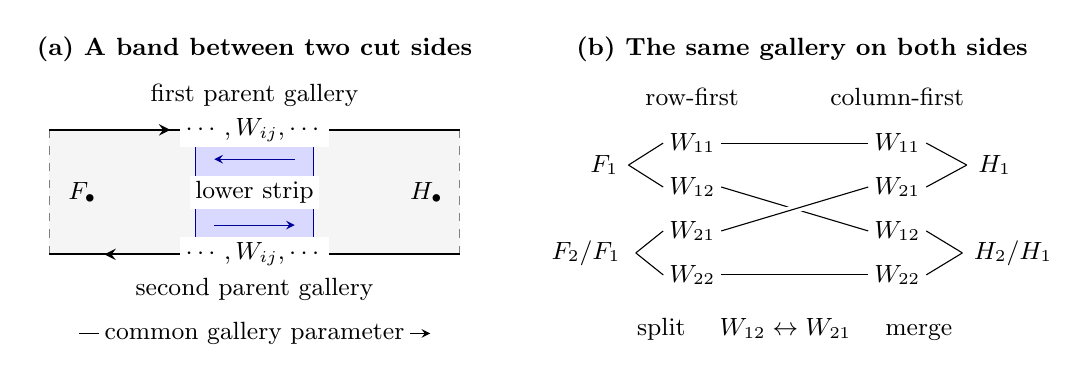
\begin{tikzpicture}[x=.93cm,y=.93cm,>=stealth,
  every node/.style={font=\small},
  block/.style={fill=white,inner sep=2pt}]
  \node[font=\small\bfseries] at (2.8,2.8) {(a) A band between two cut sides};
  \fill[gray!8] (0,0) rectangle (5.6,1.7);
  \draw[dashed,gray] (0,0)--(0,1.7) (5.6,0)--(5.6,1.7);
  \fill[blue!15] (2.0,0) rectangle (3.6,1.7);
  \draw[blue!60!black] (2.0,0)--(2.0,1.7) (3.6,0)--(3.6,1.7);
  \draw[thick] (0,1.7)--(5.6,1.7) (0,0)--(5.6,0);
  \draw[->,thick] (.75,1.7)--(1.65,1.7);
  \draw[<-,thick] (.75,0)--(1.65,0);
  \draw[<-,blue!60!black] (2.25,1.3)--(3.35,1.3);
  \draw[->,blue!60!black] (2.25,.4)--(3.35,.4);
  \node[block] at (2.8,1.7) {$\cdots,W_{ij},\cdots$};
  \node[block] at (2.8,0) {$\cdots,W_{ij},\cdots$};
  \node at (2.8,2.17) {first parent gallery};
  \node at (2.8,-.47) {second parent gallery};
  \node at (.45,.85) {$F_\bullet$};
  \node at (5.15,.85) {$H_\bullet$};
  \node[align=center,fill=white,inner sep=2pt] at (2.8,.85)
       {lower strip};
  \draw[->] (.4,-1.08)--(5.2,-1.08);
  \node[fill=white,inner sep=2pt] at (2.8,-1.08)
       {common gallery parameter};

  \begin{scope}[xshift=7.0cm]
    \node[font=\small\bfseries] at (2.75,2.8) {(b) The same gallery on both sides};
    \node at (.05,1.22) {$F_1$};
    \node at (-.2,.02) {$F_2/F_1$};
    \node[block] (l11) at (1.25,1.52) {$W_{11}$};
    \node[block] (l12) at (1.25,.92) {$W_{12}$};
    \node[block] (l21) at (1.25,.32) {$W_{21}$};
    \node[block] (l22) at (1.25,-.28) {$W_{22}$};
    \node[block] (r11) at (4.05,1.52) {$W_{11}$};
    \node[block] (r21) at (4.05,.92) {$W_{21}$};
    \node[block] (r12) at (4.05,.32) {$W_{12}$};
    \node[block] (r22) at (4.05,-.28) {$W_{22}$};
    \node at (5.38,1.22) {$H_1$};
    \node at (5.63,.02) {$H_2/H_1$};
    \draw (.38,1.22)--(l11.west) (.38,1.22)--(l12.west);
    \draw (.48,.02)--(l21.west) (.48,.02)--(l22.west);
    \draw (l11.east)--(r11.west) (l22.east)--(r22.west);
    \draw (l12.east)--(r12.west);
    \draw[preaction={draw=white,line width=3pt}]
          (l21.east)--(r21.west);
    \draw (r11.east)--(5.0,1.22) (r21.east)--(5.0,1.22);
    \draw (r12.east)--(4.94,.02) (r22.east)--(4.94,.02);
    \node at (1.25,2.15) {row-first};
    \node at (4.05,2.15) {column-first};
    \node[align=center] at (2.65,-1.02)
      {split\quad\ $W_{12}\leftrightarrow W_{21}$\quad\ merge};
  \end{scope}
\end{tikzpicture}

\caption{Replacing a cut band by lower-rank strips.
Both parent sides carry the same gallery from $F_\bullet$ to
$H_\bullet$, with the same array $(m_{ij})$.
Panel (a) displays one strip occurrence; the arrows on its boundary
oppose the parent boundary arrows.  The galleries use a common
parameter, independently of those boundary orientations.
Panel (b) shows the two-by-two sorting pattern, with $F_2=H_2=V$.
Splits and merges
are performed on both parent sides, using transverse seams on the
relevant strips.  The crossing represents an interchange and adds
no incidence between strips.  This is an incidence schematic,
not a planar embedding of the whole diagram.}
\label{fig:band-gallery}
\end{figure}

All strips inherit the band orientation.  Their long-side boundary
orientations are opposite to those of the corresponding parents,
and the short-end attachments sew opposite orientations.  Thus the
result is again an oriented surface diagram.  Its only rank-$n$
facets are disks, possibly with punctures.  Every new strip has rank
less than $n$, since it refines a child of a proper seam.  Zero
blocks can be deleted.

We verify reconstruction before applying density.  A solution of
the cut diagram gives two pairs of flags, one on each side of the
band.  The old child transports prescribe isomorphisms on their
$F$-graded and $H$-graded modules.  Transverse split and merge seams
make those isomorphisms preserve the refinements.  Transports on the
fully refined strips and the natural maps at interchanges make
them agree on the double-graded modules.  Lemma~\ref{lem:two-flags}
therefore supplies a full isomorphism respecting the entire gallery,
not just its endpoint flags.  Use it to sew back
the rank-$n$ band.  The old seam flags extend across its short ends.
Different bands give independent matching choices.

Conversely, transport the two endpoint flags of an old solution
into a band.  Their intersection ranks specify one of finitely many
arrays; a simultaneous splitting gives its two-flag sequences and
all the strips, matched by the old band transport.  This produces
a cut solution reconstructing the old one.  The matching choices
form locally affine bundles by Lemma~\ref{lem:two-flags}, and over
integral cut solutions they have dense integral parameters.  Thus
Lemma~\ref{lem:density-transfer} reduces the problem to diagrams
whose maximal-rank facets are disks.  The added topology of the
lower-rank facets is retained and causes no restriction in the
induction hypothesis.

\subsection{Replacing a disk by a subspace and a quotient}

Let $V$ be one rank-$n$ disk.  At one starting boundary interval,
choose a nonzero proper prefix of its seam flag, ending at index $k$.
Such a prefix exists because the seam is proper.  In an old solution
this subspace extends to a parallel subsystem $U$ throughout the
punctured disk, because every puncture monodromy is scalar.  Put
$Q=V/U$.  Both ranks are less than $n$, and both systems have the
same scalar puncture monodromies as $V$.

The prefix will make the reconstruction close around the boundary.
At this interval the induced flags satisfy $Q_i=0$ for $i\leq k$
and $U_i=U$ for $i\geq k$.  Once these flags and their identified
quotients are fixed, they have a unique lift in $U\oplus Q$: before
$k$ it is the given flag in $U$, and after $k$ it is the inverse
image of the flag in $Q$.  Equivalently, the stabilizer in
Lemma~\ref{lem:filtered-lift} is all of $H=\Hom(Q,U)$.
These zero-rank conditions will be part of the chosen lower diagram,
so the unique starting lift exists for every lower solution, not only
for one extracted from an old solution.

On an interval with old seam list $W_1,\ldots,W_m$, the old flag
induces flags on $U,Q$ and exact sequences
\begin{equation}\label{eq:boundary-exact-sequences}
 0\longrightarrow U_i/U_{i-1}\longrightarrow W_i
 \longrightarrow Q_i/Q_{i-1}\longrightarrow0.
\end{equation}
Choose the ranks of all these modules, and of the modules at the
finitely many vertices below.  There are finitely many possibilities;
we use the possibilities arising from old complex solutions.  The
actual construction of the lower diagram depends only on these
ranks, not on the old solution.  In particular, at the starting
interval the $Q$-graded pieces have rank zero for $i\leq k$, and the
$U$-graded pieces have rank zero for $i>k$.
Intersections and projection images are extracted only from complex
solutions.  Integral reconstruction will instead use the specified
free child modules; it does not require intersections of arbitrary
$R$-lattices to be free.

Replace $V$ by two disks $U,Q$, with the same orientation and scalar
punctures.  On a regular interval replace its seam by
\[
 U:(u_1,\ldots,u_m),\qquad
 Q:(q_1,\ldots,q_m),\qquad
 W_i:(u_i,q_i).
\]
Here $u_i$ is an actual strip joining the $U$ side to the $W_i$
side, as child on both, and $q_i$ similarly joins $Q$ to $W_i$.
Its transport gives the maps in
\eqref{eq:boundary-exact-sequences}.  Along an unmarked seam circle
these may be cyclic strips.  The old parent and child have opposite
boundary orientations, so the strips sew with the required
orientations.

We describe the two vertex replacements.  In these descriptions,
time increases along the positive boundary orientation of $V$, and
along those of $U,Q$.  It therefore runs opposite to the old child
boundary orientation.  Unaffected strips and lists continue.

Each replacement has a common reconstruction requirement.  At a split,
the coarse quotient is $W$ with its internal flag; at an interchange,
it is $A\oplus B$ with its given decomposition.  The lower data must
supply an exact sequence with this middle term whose restrictions
are the exact data on both neighboring intervals.
Lemma~\ref{lem:filtered-lift} will then extend an incoming interval
lift to the vertex, and that choice will determine the outgoing lift.

\subsubsection*{A split or merge}

Suppose an old block $W$ splits into $W'_1,\ldots,W'_s$.  Before
the event its list is $W:(w,q)$.  Split the $w,q$ connections into
$w_1,\ldots,w_s$ and $q_1,\ldots,q_s$ by transverse seams, refining
the lists at both ends of each connection.  On $W$, use the
two-flag sequence to interleave them as
\[
 w_1,q_1,\ldots,w_s,q_s.
\]
Merge each pair in this list to $W'_j$, introducing the side of
$W'_j$ through the merge vertex and its seam $W'_j:(w_j,q_j)$.
The resulting list on $W$ continues onto the old additional seam
$W:(W'_1,\ldots,W'_s)$.

At this merge vertex the $W'_j$ corner joins its occurrence as a
child of $W$ to its occurrence as parent of $w_j,q_j$.  The strip
boundaries formerly at $W$ continue at $W'_j$, and their other ends
remain at $U,Q$.  This describes all germ pairings.  The $W$ lists
run opposite to its boundary orientation toward the old side seam;
the $W'_j$ sides run into that seam as children and out along their
new strips as parents.  Hence the orientations agree.  Reverse
this construction for an old merge.

Lemma~\ref{lem:two-flags} says exactly what the construction records:
the flag of $W$ with two pieces $w,q$ is compared with its flag
having pieces $W'_j$.  Their intersections induce the refined flags
on $U,Q$, and the matched double-graded maps give the exact sequences
for the $W'_j$.  Every old complex solution admits this replacement.
Conversely, any lower solution supplies these compatible refined
exact sequences, including all their identified quotients.

Here the seam $W:(w,q)$ supplies the coarse exact sequence, and the
retained seam $W:(W'_1,\ldots,W'_s)$ supplies its internal flag.
The two-flag gallery makes their induced fine quotient maps agree.
Thus every lower solution supplies the coarse exact sequence with
middle term $W$ and its fixed internal flag, not only the sequences on
the fine quotients $W'_j$.  The restriction of a vertex lift to the coarse
interval is the identity.  On the fine interval we forget the full
identification with $W$.  For the exact sequences
$0\to w_j\to W'_j\to q_j\to0$, free compatible splittings give
\[
 K_{\rm interval}/K_{\rm coarse}
     =\bigoplus_{k<j}\Hom_R(q_j,w_k).
\]
The restriction to that interval is therefore an affine surjection
with free integral parameters.  The same two restrictions handle the
reverse merge.

\subsubsection*{An interchange and the negative scalar}

Now suppose the old event interchanges $A,B$.  Their coarsened
quotient of $V$ is identified with $A\oplus B$.  In an old solution
write $U_*\subset A\oplus B$ and $Q_*=(A\oplus B)/U_*$ for the
induced subquotients.  Put
\[
 a=U_*\cap A,\quad b=U_*\cap B,\quad
 \widetilde a=\operatorname{pr}_A(U_*),\quad
 \widetilde b=\operatorname{pr}_B(U_*).
\]
The modules $\widetilde a/a$ and $\widetilde b/b$ have the same rank,
denoted $h$.  Put $x=A/\widetilde a$ and $y=B/\widetilde b$.
The required before and after lists are
\[
\begin{array}{c|cc}
 &\text{before}&\text{after}\\ \hline
 U_*&a,\widetilde b&b,\widetilde a\\
 Q_*&A/a,y&B/b,x\\
 A&a,A/a&\widetilde a,x\\
 B&\widetilde b,y&b,B/b.
\end{array}
\]
These symbols name ranks and strip occurrences in the new diagram;
the intersection description explains how every old solution
determines such data.

Split the incoming $\widetilde b$ connection into $b,h$, and the
incoming $A/a$ connection into $h,x$.  The four lists become
\[
 U_*:(a,b,h),\quad Q_*:(h,x,y),\quad
 A:(a,h,x),\quad B:(b,h,y).
\]
Interchange $a,b$ on $U$ and $x,y$ on $Q$, leaving those connections
unchanged.  Replace the two $h$ connections
\[
 (U,B),(Q,A)\qquad\text{by}\qquad(U,A),(Q,B)
\]
using one punctured disk of rank $h$, with scalar monodromy $-I$.
Its boundary contacts, all as child, occur in the cyclic order
$U,B,Q,A$.  Along $U$ it runs from positive to negative time,
then crosses the incoming $(U,B)$ strip end; along $B$ it runs
from negative to positive time, then crosses the outgoing $(B,Q)$
end; along $Q$ it runs from positive to negative time, then crosses
the incoming $(Q,A)$ end; along $A$ it runs from negative to positive
time, then crosses the outgoing $(A,U)$ end.  This specifies the
oriented sewing to all four strip ends.  Finally merge $a,h$ to
$\widetilde a$ and $h,y$ to $B/b$.  If $h=0$, delete this disk.

The lower solution provides maps $p_A:U_*\to A$, $p_B:U_*\to B$,
$i_A:A\to Q_*$ and $i_B:B\to Q_*$, with the images and kernels
specified in the table.  Write
\[
 h_U=U_*/(a\oplus b),\qquad
 h_A=\widetilde a/a,\qquad h_B=\widetilde b/b,\qquad
 h_Q=\operatorname{im}i_A\cap\operatorname{im}i_B.
\]
These are the rank-$h$ subquotients at the four contacts.  The maps
$p_A,p_B$ induce isomorphisms from $h_U$ to $h_A,h_B$, and
$i_A,i_B$ induce isomorphisms from $h_A,h_B$ to $h_Q$.
Figure~\ref{fig:swap-disk} displays the two resulting paths from
$h_U$ to $h_Q$.

\begin{figure}[ht]
\centering
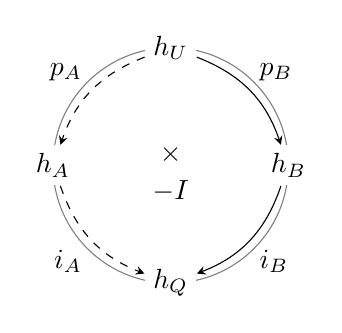
\begin{tikzpicture}[scale=1.15,>=stealth]
  \draw[gray] (0,0) circle (1.3);
  \node[fill=white,inner sep=3pt] (u) at (0,1.3) {$h_U$};
  \node[fill=white,inner sep=3pt] (b) at (1.3,0) {$h_B$};
  \node[fill=white,inner sep=3pt] (q) at (0,-1.3) {$h_Q$};
  \node[fill=white,inner sep=3pt] (a) at (-1.3,0) {$h_A$};
  \draw[->] (u) to[bend left=25] node[above right] {$p_B$} (b);
  \draw[->] (b) to[bend left=25] node[below right] {$i_B$} (q);
  \draw[->,dashed] (u) to[bend right=25] node[above left] {$p_A$} (a);
  \draw[->,dashed] (a) to[bend right=25] node[below left] {$i_A$} (q);
  \node at (0,0.12) {$\times$};
  \node at (0,-0.28) {$-I$};
\end{tikzpicture}

\caption{The four contacts of the punctured $h$-disk.
The symbols denote the corresponding $h$-subquotients and the
maps they inherit.  The two paths from $h_U$ to $h_Q$ differ by
the monodromy $-I$, so $i_Ap_A+i_Bp_B=0$.}
\label{fig:swap-disk}
\end{figure}

The two composites $i_Ap_A,i_Bp_B$ factor through $h_U$ to $h_Q$.
They are opposite, because they are the two transports around the
punctured $h$-disk.  Hence the following sequence is a complex:
\begin{equation}\label{eq:swap-exact-sequence}
 0\longrightarrow U_*
 \xrightarrow{(p_A,p_B)}A\oplus B
 \xrightarrow{(i_A,i_B)}Q_*\longrightarrow0
\end{equation}
It is exact over $R$ as well as over $\C$.  The kernels of $p_A,p_B$
are respectively $b,a$, and their intersection is zero by the
interchange on $U$.  The images of $i_A,i_B$ span $Q_*$ because
their $x,y$ quotients are complementary.  If
$i_A(z)+i_B(t)=0$, projection modulo $\operatorname{im}i_A$ gives
$t\in\widetilde b$.  Lift $t$ under $p_B$ and subtract the image
of that lift; the remaining vector is in $\ker i_A=a$, which is
again in the image of $U_*$.  The needed lifts exist over $R$
because the named quotients are free.

For clarity, in split coordinates the maps are
\begin{align*}
 U_*&=a\oplus b\oplus h,&A&=a\oplus h\oplus x,\\
 Q_*&=h\oplus x\oplus y,&B&=b\oplus h\oplus y,\\
 p_A(a,b,h)&=(a,h,0),&p_B(a,b,h)&=(b,h,0),\\
 i_A(a,h,x)&=(h,x,0),&i_B(b,h,y)&=(-h,0,y).
\end{align*}
Thus the scalar $-I$ supplies exactly the sign needed in
\eqref{eq:swap-exact-sequence}; no division by $2$ is involved.
Conversely, any old exact sequence with the induced flags gives
the refinements and maps above, and its two induced $h$-maps have
this opposite sign.  They therefore extend over the punctured disk.

The exact sequence with middle term $A\oplus B$ is the coarse vertex
data required for reconstruction.  In the displayed free coordinates,
forgetting its full identification permits the additional stabilizer
block $\Hom_R(y,a)$ on the incoming interval and $\Hom_R(x,b)$ on
the outgoing interval.  All unchanged blocks cancel from these
quotients.  Each restriction is considered separately: split its
refined flags on $U,Q$ and group the free summands to obtain the
coarse flags.  Both restrictions are affine surjections with free
integral parameters.  No simultaneous choice of both interval lifts
is required.

All replacements occur in separate side intervals and corner
neighborhoods.  They preserve the other seams of every lower-rank
facet, including repeated occurrences of the same facet.  Parallel
maps on the strips extend across the specified cross sections, so
the construction also applies to cyclic boundary lists.

\subsection{Reconstruction and closure around a disk}

We now reconstruct a disk from an arbitrary solution of its lower
diagram.  Put $V=U\oplus Q$.  All puncture monodromies are the
prescribed scalars, so this is a local system with the required
monodromy.  Moreover $H=\Hom(Q,U)$ is constant on the punctured
disk: the identical scalar monodromies of $U,Q$ act trivially on it.

The starting interval has the unique lift already established.
Continue it by parallel transport to the first vertex.  The relevant
vertex construction gives an affine space of extensions of this
incoming lift.  Choose one and restrict it to the outgoing interval,
then repeat around the boundary.  Every step is surjective with affine
fiber, and over integral lower data that fiber has free integral
parameters.  On return, the starting interval still has just one lift,
so the propagated lift agrees with it automatically.  This includes
all identified quotients: they belong to the lift spaces and are not
additional data to be matched afterward.  With no vertices, the same
unique lift is parallel around the unmarked seam circle.  Thus closure
imposes no further equation.

For each fixed rank pattern these successive choices form a finite
tower of locally affine bundles over the lower solution variety.
Indeed the flags have constant ranks, so they can be split locally,
and the preceding matrix-block descriptions give each event fiber.
Every integral lower solution admits integral choices, dense in those
fibers by Lemma~\ref{lem:integral-parameters}.  Conversely, every old
complex solution is recovered from its induced lower data and its
original lifts, up to the allowed frame changes.  Its disk local
system is isomorphic to $U\oplus Q$ because all puncture generators
act by the prescribed scalars.

Perform the construction on every rank-$n$ disk.  No new rank-$n$
facet has been introduced.  After normalizing zero blocks and
identity seams, the induction hypothesis gives density on each
resulting lower diagram.  Lemma~\ref{lem:density-transfer} gives
density on the disk diagrams and then on the original nonclosed
diagram.  This proves Proposition~\ref{prop:nonclosed-reduction}.

Closed maximal-rank facets remain.  The next two sections treat their
scalar-monodromy equations; after the closed-density lemma we assemble
the full induction proving Theorem~\ref{thm:diagram-density}.

\section{Closed surfaces with scalar monodromy}
\label{sec:surfaces}

Closing a surface with prescribed scalar monodromies leads to a product
of commutators.  We first settle the case of genus one, and then prove
the irreducibility needed for the higher-genus argument.  For
\(n\geq1\), \(g\geq0\), and \(c\in\C^\times\), write
\[
 \mathcal R_{n,g}(c)=
 \left\{(A_1,B_1,\ldots,A_g,B_g)\in\GL_n(\C)^{2g}:
       \prod_{j=1}^g[A_j,B_j]=cI_n\right\},
 \qquad [A,B]=ABA^{-1}B^{-1}.
\]
As throughout the paper, this is a reduced variety.  Taking determinants
shows that it is empty unless \(c^n=1\).  For genus zero it is a point
if \(c=1\), and is empty otherwise.  For rank one and \(c=1\), it is
the torus \((\C^\times)^{2g}\).

\subsection{Genus one}

The density of simultaneously diagonalizable commuting pairs goes back
to Motzkin and Taussky~\cite{MotzkinTaussky1955}; see also
Gerstenhaber~\cite{Gerstenhaber1961} and Guralnick~\cite{Guralnick1992}.
We use the regular-centralizer proof described by Guralnick and
Sethuraman~\cite[Section~3, Proposition~6]{GuralnickSethuraman2000},
then record its integral consequence over the full ring in use here.

\begin{lemma}\label{lem:commuting-density}
Let \(R\subset\C\) be an infinite domain with infinitely many units.
Then the pairs of commuting matrices in \(\GL_d(R)\) are Zariski dense
in the variety of commuting pairs in \(\GL_d(\C)\).
\end{lemma}

\begin{proof}
Call a matrix regular if its minimal polynomial has degree \(d\).
The centralizer of any matrix \(C\) contains a regular matrix \(E\):
in a Jordan basis for \(C\), take \(E\) to have blocks
\(\mu_i I+N_i\), where \(N_i\) is the nilpotent Jordan block of the
corresponding size and all \(\mu_i\) are distinct.  The minimal
polynomial of \(E\) then has degree \(d\).

Given a commuting invertible pair \((C,D)\), the matrix
\(D+tE\) is regular and invertible for generic \(t\).
Indeed regularity is open and holds near infinity on this line, since
\(E+t^{-1}D\) tends to \(E\); the determinant polynomial is nonzero
at \(t=0\).  Fix such a \(t\).  The centralizer of the regular matrix
\(D_t=D+tE\) is \(\C[D_t]\): a commuting map is determined by its
value on a cyclic vector, and that value is achieved by a polynomial
in \(D_t\).  Thus \(C=f(D_t)\) for a polynomial \(f\).
Perturbing \(D_t\) to matrices \(D'\) with distinct
eigenvalues, while keeping both \(D'\) and \(f(D')\) invertible,
approximates \((C,D_t)\) by simultaneously diagonalizable pairs.
Letting \(t\) tend to zero proves their density among all commuting
invertible pairs.

The group \(\GL_d(R)\) is Zariski dense in \(\GL_d(\C)\).
Its closure contains all elementary unipotent groups, since \(R\)
is infinite, and the diagonal torus, since \(R^\times\) is infinite;
these generate \(\GL_d\).  Thus the integral points in the domain of
\[
 \GL_d\times(\mathbb G_m)^d\times(\mathbb G_m)^d
 \longrightarrow \GL_d^2,
 \qquad
 (P,u,v)\longmapsto
 \bigl(P\operatorname{diag}(u)P^{-1},
       P\operatorname{diag}(v)P^{-1}\bigr)
\]
are dense.  Their images are integral commuting pairs, and the image
is exactly the simultaneously diagonalizable locus.  Notice that
\(P^{-1}\) has entries in \(R\) when \(P\in\GL_d(R)\).
\end{proof}

\begin{lemma}\label{lem:torus-density}
Let \(R\subset\C\) be an infinite domain with infinitely many units.
If \(c\in R\) is a root of unity and \(c^n=1\), then
\(\mathcal R_{n,1}(c)(R)\) is Zariski dense in
\(\mathcal R_{n,1}(c)\).
\end{lemma}

\begin{proof}
Put \(m=\operatorname{ord}(c)\), so \(m\mid n\).  The equation is
\(AB=cBA\).  Therefore \(B\) carries the generalized
\(\lambda\)-eigenspace of \(A\) onto its generalized
\(c\lambda\)-eigenspace.  All eigenvalues are nonzero, so each orbit
under multiplication by \(c\) has length \(m\).
Let \(V_0\) be the sum of one generalized eigenspace from each orbit,
and identify \(V_j=B^jV_0\) with \(V_0\), for \(0\leq j<m\),
using \(B^j\).  These spaces give a direct sum of \(\C^n\), and
\(\dim V_0=n/m\).  In these coordinates the matrices have the form
\[
 A=\operatorname{diag}(C,cC,\ldots,c^{m-1}C),\qquad
 B(v_0,\ldots,v_{m-1})=(Dv_{m-1},v_0,\ldots,v_{m-2}),
\]
where \(C=A|_{V_0}\) and \(D=B^m|_{V_0}\) commute.
Conversely, any commuting invertible \(C,D\) give a solution by these
formulas.  In particular the wrap-around relation uses precisely
\(CD=DC\) and \(c^m=1\).

We have obtained a surjective morphism from
\(\GL_n\) times the variety of commuting invertible
\((n/m)\)-dimensional pairs to \(\mathcal R_{n,1}(c)\), by the displayed
construction followed by conjugation.  Lemma~\ref{lem:commuting-density}
and density of \(\GL_n(R)\) give a dense set of integral points in its
domain.  Their images are integral solutions.
\end{proof}

In our application \(R=\cO_F\), and the unit \(1+\sqrt2\) has
infinite order.  Thus these lemmas, as well as the rank-one torus
case, apply over the fixed ring already chosen.

\subsection{Irreducibility in higher genus}

The proof below follows the character-count and Lang--Weil method of
Liebeck--Shalev~\cite[Section~7, Lemma~7.1 and the proof of Theorem~1.8]{LiebeckShalev2005}.
We give the elementary
estimates for \(\SL_n\), and use a lower bound for the dimension of
every component to obtain irreducibility of the entire fiber.

\begin{proposition}\label{prop:surface-irreducibility}
For \(n\geq2\), \(g\geq2\), and \(c^n=1\), the variety
\(\mathcal R_{n,g}(c)\) is irreducible of dimension
\((2g-1)n^2+1\).
\end{proposition}

\begin{proof}
For a field \(k\) and a scalar \(c\in k^\times\) with \(c^n=1\),
let \(\mathcal S_k(c)\) denote the fiber obtained by imposing
determinant one on every handle matrix.  First work over a finite
field \(k=\mathbb F_q\), and put
\(G=\SL_n(\mathbb F_q)\) and \(z=cI_n\).
We need two elementary estimates:
\begin{equation}\label{eq:surface-character-bounds}
 |\operatorname{Irr}(G)|=O_n(q^{n-1}),\qquad
 \chi(1)\geq\frac{q^{n-1}-1}{2}
 \quad\text{for every nontrivial }\chi\in\operatorname{Irr}(G).
\end{equation}

For the first estimate, there are \(q^{n-1}\) possible monic
characteristic polynomials of degree \(n\) and determinant one.
For each polynomial, rational canonical form is specified by a
partition for each of its distinct irreducible factors.  There are
at most \(n\) factors, and the relevant partition numbers are bounded
in terms of \(n\).  Thus there are \(O_n(q^{n-1})\)
\(\GL_n(\mathbb F_q)\)-classes of determinant one.
Such a class splits into
\[
 [\mathbb F_q^\times:
       \det C_{\GL_n(\mathbb F_q)}(x)]\leq n
\]
classes in \(G\), since the centralizer contains the scalar matrices,
whose determinants are the \(n\)-th powers.  This bounds the number
of conjugacy classes in \(G\), hence its number of irreducible characters.

For the degree estimate, restrict a nontrivial irreducible complex
representation to the abelian subgroup
\[
 U=\left\{\begin{pmatrix}1&v\\0&I_{n-1}\end{pmatrix}:
                  v\in\mathbb F_q^{n-1}\right\}.
\]
A nontrivial character of \(U\) must occur: otherwise the representation
would be trivial on \(U\) and on all its conjugates, which generate
\(G\).  Every character in its orbit under the normalizer also occurs.
For \(n\geq3\), the subgroup
\(\operatorname{diag}(1,\SL_{n-1}(\mathbb F_q))\) acts transitively
on the nontrivial characters of \(U\).  Indeed a fixed nontrivial
additive character of the prime field, composed with the field trace, identifies them
with the nonzero vectors in the dual of \(\mathbb F_q^{n-1}\).
This gives the stronger bound \(q^{n-1}-1\).
For \(n=2\), conjugation by \(\operatorname{diag}(a,a^{-1})\)
acts by square scalings; a nontrivial character has an orbit of size
\((q-1)/\gcd(2,q-1)\).  This proves
\eqref{eq:surface-character-bounds}, including the small fields.

The Frobenius commutator formula now gives the number of solutions as
\begin{equation}\label{eq:surface-frobenius}
 |G|^{2g-1}\sum_{\chi\in\operatorname{Irr}(G)}
          \frac{\chi(z^{-1})}{\chi(1)^{2g-1}}
 =|G|^{2g-1}\bigl(1+O_n(q^{-(n-1)})\bigr).
\end{equation}
For completeness, the central element
\(T=\sum_{a,b\in G}[a,b]\in\C[G]\) acts on an irreducible
representation of degree \(d\) as \(|G|^2/d^2\), by Schur
orthogonality.  Expanding \(T^g\) in the central idempotents
\[
 e_\chi=\frac{\chi(1)}{|G|}
             \sum_{x\in G}\chi(x^{-1})x
\]
and taking its coefficient at \(z\) proves the first expression
in \eqref{eq:surface-frobenius}; see also
\cite[Lemma~3.1(i)]{LiebeckShalev2005}.
Centrality gives \(|\chi(z^{-1})|=\chi(1)\).  Since \(g\geq2\),
the absolute contribution of all nontrivial characters is at most
\(\sum_{\chi\ne1}\chi(1)^{-2}=O_n(q^{-(n-1)})\), by
\eqref{eq:surface-character-bounds}.

Let \(\mathcal S=\mathcal S_{\overline{\mathbb F}_q}(c)\), and set
\(D=(2g-1)(n^2-1)\).  The target \(\SL_n\) of the product-of-commutators
map is smooth of dimension \(n^2-1\).  Its fiber is therefore locally
cut out in the smooth variety \(\SL_n^{2g}\) by \(n^2-1\) equations.
The principal ideal theorem implies that every component of
\(\mathcal S\) has dimension at least \(D\).
On the other hand,
\[
 |\SL_n(\mathbb F_q)|
       =q^{n^2-1}\prod_{i=2}^n(1-q^{-i}),
\]
so \eqref{eq:surface-frobenius} says that its fiber has
\(q^D(1+o(1))\) points as \(q\) tends to infinity through extensions
of any fixed field of definition.

Pass to a finite field \(\mathbb F_Q\) over which \(c\) and all
geometric components are defined, and write \(q=Q^m\).
For a fixed geometrically irreducible component of dimension \(d\),
the Lang--Weil estimate is \(q^d+O(q^{d-1/2})\), with a constant
independent of \(m\); a fixed variety of dimension at most \(d-1\)
has \(O(q^{d-1})\) points~\cite{LangWeil1954}; see also
\cite[Theorem~7.7.1]{Poonen2017}.
The character count holds over every one of these extension fields.
It therefore first rules out components of dimension greater than
\(D\).  All components consequently have dimension
\(D\).  If there are \(e\) of them, the same estimate, together with
the smaller dimensions of their pairwise intersections, gives
\[
 |\mathcal S(\mathbb F_q)|=e q^D+O(q^{D-1/2}).
\]
Comparison with the preceding count yields \(e=1\).  The counts
are positive over sufficiently large extensions, so the fiber is
nonempty.  We have proved geometric irreducibility, including when
the initial field is small.

This also proves irreducibility in characteristic zero.  The
characteristic-zero fiber is nonempty: take the clock-and-shift
solution in Lemma~\ref{lem:torus-density}, normalize its two
determinants by complex scalar roots, and put identities on the
remaining handles.  If the fiber were reducible,
after extending the number field containing \(c\), the geometric
generic fiber would contain two disjoint nonempty open subsets,
obtained by removing the other irreducible components.  Spread their
finite defining data over a localization of its ring of integers.
After shrinking this base, the two opens remain disjoint and both
have nonempty fibers.  Here constructibility of images ensures that
an open which meets the generic fiber meets every fiber over some
nonempty open of the base.  A closed fiber would thus have two
disjoint nonempty geometric opens, contradicting the irreducibility
just proved.  The characteristic-zero dimension is \(D\): after
shrinking the arithmetic base, fiber dimension agrees with generic
fiber dimension, whereas the closed fibers all have dimension \(D\).

Finally, multiplication of the \(2g\) handle matrices by independent
central scalars gives a surjective morphism
\[
 \mathcal S_{\C}(c)\times(\mathbb G_m)^{2g}
       \longrightarrow\mathcal R_{n,g}(c).
\]
Surjectivity follows by taking an \(n\)-th root of each determinant.
The domain is irreducible and the fibers are finite, consisting of
the scalar choices of these roots.  The image is therefore
irreducible of dimension \(D+2g=(2g-1)n^2+1\).
\end{proof}

Proposition~\ref{prop:surface-irreducibility} is a geometric statement.
The roots used in its last paragraph are taken in \(\C\); the
arithmetic passage to determinant one over a single number field
will be treated separately.

\section{From one spectrum to a closed surface}
\label{sec:dynamics}

The remaining step in the diagram induction concerns a closed facet.
Cutting a nonseparating circle reduces it to a facet with boundary, but
prescribes the spectrum of the gluing monodromy.  We first obtain density
with this spectrum fixed.  A Dehn twist then supplies the missing
directions.

Multiplication by a centralizer element is the algebraic form of
the generalized twist motions described by
Goldman~\cite[Section~4.6]{Goldman1986}.  We use the matrix relation
directly, then verify the needed torus closure and tangent directions
at an explicit representation.

\begin{lemma}\label{lem:closed-density}
Let $2\le n\le r$, $g\ge2$, and let $c\in F$ satisfy $c^n=1$.
Assume that integral solutions are dense for every normalized diagram
of ranks at most $n$ whose rank-$n$ facets have nonempty boundary.
Then $\mathcal R_{n,g}(c)(R)$ is Zariski dense in
$\mathcal R_{n,g}(c)$.
\end{lemma}

\begin{proof}
Write $V=\mathcal R_{n,g}(c)$ and let $D$ be the Zariski closure of its
integral points.  By Proposition~\ref{prop:surface-irreducibility}, $V$
is irreducible.

\smallskip\noindent\emph{Integral gluing at a fixed spectrum.}
Choose
\[
 \alpha_i=\zeta^{\,i-1}\qquad(1\le i\le n).
\]
These numbers are distinct and their pairwise differences are units of
$R$, by Lemma~\ref{lem:unit-spectrum}.  We first show that $D$ contains
the entire fiber
\[
 V_\alpha=\{(A_j,B_j)\in V:
            \det(XI-A_1)=\prod_{i=1}^n(X-\alpha_i)\}.
\]

Represent $V$ by a genus-$g$ facet with one puncture of scalar
monodromy $c^{-1}$, so that the surface relation is
$\prod_j[A_j,B_j]=cI$.
Cut this surface along the circle represented by $A_1$.  On each new
boundary, require a full flag with successive scalar monodromies
$\alpha_1,\ldots,\alpha_n$, using rank-one punctured disk caps.  Here
the two loops are read in the same original direction; their induced
boundary orientations are opposite, so one reverses the cap scalar
when necessary.  The new seams have $n>1$ rank-one children, so they
are proper; the resulting rank-$n$ facet has boundary.  The
hypothesis gives density of integral solutions on this cut diagram.

To reglue, choose an isomorphism between the two boundary systems.
Because the eigenvalues are distinct, the choices form a torsor for
$(\mathbb G_m)^n$, by matching corresponding eigenlines.  They vary
locally algebraically with the cut solution, so their projection to
the cut solution variety is open and surjective.
This description also holds over $R$.  Indeed the spectral projectors
\begin{equation}\label{eq:spectral-projectors}
 E_i(A)=\prod_{j\ne i}\frac{A-\alpha_jI}{\alpha_i-\alpha_j}
 \in M_n(R)
\end{equation}
split off the eigenmodules.  Write $F_\bullet$ for the prescribed
flag.  The projector $E_i$ is zero on $F_{i-1}$ and on $R^n/F_i$:
on each of their graded pieces its action is zero, so its induced
action is both nilpotent and idempotent.  It induces the identity on
$F_i/F_{i-1}$.  Hence its image is isomorphic to that graded line,
which is free because it is identified with a framed cap fiber.
Thus every integral cut
solution has gluing choices, and in these bases the integral choices
are $(R^\times)^n$, a dense subset of the gluing torus by
Lemma~\ref{lem:integral-parameters}.
The open-projection density principle therefore gives dense integral
glued solutions.  Conversely, every point of $V_\alpha$ admits these
ordered eigenflags and cap frames, and is recovered by gluing, up to
frame changes.  Frame changes over $R$ are dense by the same lemma.  Hence
$V_\alpha\subset D$.

\smallskip\noindent\emph{Torus saturation by Dehn twists.}
The automorphisms
\[
 \tau^{\pm1}(A_1,B_1,A_2,B_2,\ldots)
       =(A_1B_1^{\pm1},B_1,A_2,B_2,\ldots)
\]
preserve $V$, since $[A_1B_1,B_1]=[A_1,B_1]$, and preserve its integral
points.  Consequently they preserve $D$.  We show that this discrete
invariance enlarges $V_\alpha$ to an analytic open subset of $V$.

Choose distinct rational primes $\beta_1,\ldots,\beta_n$.  They are
multiplicatively independent.  Let $P$ be the cyclic permutation
matrix $Pe_i=e_{i+1}$, with indices modulo $n$.  The point $x_0\in V$
given by
\begin{equation}\label{eq:twist-test-point}
 \begin{aligned}
 A_1&=\operatorname{diag}(\alpha_1,\ldots,\alpha_n),&
 B_1&=\operatorname{diag}(\beta_1,\ldots,\beta_n),\\
 A_2&=P,&
 B_2&=\operatorname{diag}(1,c^{-1},\ldots,c^{1-n})
 \end{aligned}
\end{equation}
and identity matrices on the other handles belongs to $V_\alpha$.
Indeed $PB_2P^{-1}=cB_2$, including the wraparound entry because
$c^n=1$.  The numbers $\beta_i$ are used only to choose this complex
point; they need not be units of $R$.

The relation map $\GL_n^{2g}\to\SL_n$ is submersive at $x_0$.
Left infinitesimal variations of $B_1$ give
$(\operatorname{Ad}_{A_1}-1)X$, spanning all off-diagonal matrices.
Diagonal variations of $B_2$ give
$(\operatorname{Ad}_P-1)H$, spanning the traceless diagonal matrices.
These span $\mathfrak{sl}_n$, so $V$ is smooth at $x_0$.
The map $\sigma$ recording the characteristic coefficients of $A_1$
is also submersive there: varying $A_1$ diagonally preserves the
relation, and the elementary-symmetric-functions map has invertible
differential at distinct eigenvalues.  Thus $V_\alpha$ is smooth near
$x_0$.

Take a small connected analytic neighborhood $U$ of $x_0$ in
$V_\alpha$.  The eigenvalues $b_i(x)$ of $B_1(x)$ and their spectral
projectors $P_i(x)$ can be labeled holomorphically on $U$, since the
spectrum at $x_0$ is simple.  For each nonzero $m\in\Z^n$, the
holomorphic function
\[
             \prod_i b_i(x)^{m_i}-1
\]
is nonzero at $x_0$.  Its zero set is therefore closed with empty
interior.  The Baire theorem implies that the points $x\in U$ with
multiplicatively independent $b_i(x)$ form a dense subset $U_0$.
For such an $x$, the powers of $B_1(x)$ are Zariski dense in its
centralizer torus: otherwise a nontrivial character of that torus
would equal one on the cyclic subgroup, giving a multiplicative relation.
Since $x\in D$ and $\tau^k(x)\in D$ for every $k\in\Z$, closedness
then gives every tuple obtained by replacing $A_1(x)$ with $A_1(x)T$,
for $T$ in this centralizer.

\smallskip\noindent\emph{A submersive family of twists.}
To extend this conclusion over all of $U$, write the centralizers in
the holomorphic form
\[
       T(x,t)=\sum_{i=1}^n t_iP_i(x),
       \qquad t\in(\C^\times)^n.
\]
Replacing $A_1(x)$ with $A_1(x)T(x,t)$ defines a holomorphic map
$\Psi:U\times(\C^\times)^n\to V$; it preserves the relation because
$T(x,t)$ commutes with $B_1(x)$.  Its values on
$U_0\times(\C^\times)^n$ lie in $D$.  Since $D$ is analytically
closed, all values of $\Psi$ lie in $D$.

At $(x_0,1)$ the directions from $U$ give $\ker(d\sigma)$.
The torus directions independently multiply the diagonal entries of
$A_1$, so their images under $d\sigma$ span its target.  Hence
$d\Psi$ is surjective.  Its image contains an analytic open subset of
$V$.  Such a subset is Zariski dense in an irreducible complex
variety, proving $D=V$.
\end{proof}

\subsection{Completion of the rank induction}

\begin{proof}[Proof of Theorem~\ref{thm:diagram-density}]
We induct on the largest facet rank $n$. The rank-zero diagram has
only empty data. Normalize zero pieces and identity seams as in
Section~\ref{subsec:identity-normalization}; solutions of the original
diagram are recovered from solutions of the normalized diagram by
integral restriction and frame changes. At rank one no proper seam
can remain, since it would have at least two positive-rank children.
Thus the normalized diagram consists of independent closed scalar
local systems. Each solution variety is empty or a torus, so the
rank-one case follows from Lemma~\ref{lem:integral-parameters}.

Now let $n\geq2$ and assume the theorem for all diagrams of ranks
less than $n$. Proposition~\ref{prop:nonclosed-reduction} proves
density for the part of the normalized diagram having no closed
rank-$n$ facet. It allows all lower-rank facets, closed or not.
Every remaining closed rank-$n$ facet is an independent factor
$\mathcal R_{n,g}(c)$, where $c$ is the inverse product of its scalar
puncture monodromies. If $c^n\ne1$, that factor is empty. Otherwise
the genus-zero factor is a point or empty,
Lemma~\ref{lem:torus-density} gives density for genus one, and
Lemma~\ref{lem:closed-density} gives it for higher genus. The
hypothesis of the last lemma is exactly the normalized nonclosed
step already established at this rank.

The product of these dense sets is dense in the normalized solution
variety. Restoring the original diagram and its frames preserves
density by Lemma~\ref{lem:integral-parameters}. This completes the
induction over the same fixed ring $R$.
\end{proof}

\section{Boundary classes and the character quotient}
\label{sec:descent}

We now apply Theorem~\ref{thm:diagram-density} to the surface underlying
the curve.  Flags encode the boundary classes by closed rank bounds.
We then make the handle determinants one and select the exact classes
on the character quotient.  This order is important: semisimplifying
a representation can decrease the Jordan blocks of a boundary
matrix.

\subsection{Flags for arbitrary Jordan classes}

Let $\overline X$ be the smooth compactification of the curve, of
genus $g$, and replace each missing point by a boundary circle.
For a prescribed boundary class, write $\nu_\lambda$ for its Jordan
partition at the eigenvalue $\lambda$, and write
\[
 c_{\lambda,1}\ge c_{\lambda,2}\ge\cdots>0
\]
for the column lengths of this partition.  Its generalized
$\lambda$-eigenspace has dimension $n_\lambda=|\nu_\lambda|$.
Order the eigenvalues once and for all.  On the boundary put a flag
whose graded pieces, in that order, have dimensions
$c_{\lambda,1},c_{\lambda,2},\ldots$ and scalar monodromy $\lambda$.
Realize each piece by a punctured disk cap, choosing the scalar
according to the meridian orientation.

Every matrix in the prescribed class admits this flag: on its
generalized $\lambda$-eigenspace use the successive kernels of powers
of $A-\lambda I$.  Conversely, any matrix with the prescribed flag
has the required characteristic polynomial and satisfies
\begin{equation}\label{eq:jordan-rank-bounds}
 \rk\bigl((A-\lambda I)^k\bigr)
 \le r-\sum_{j=1}^k c_{\lambda,j}
 \qquad(\lambda\text{ prescribed},\ k\ge1),
\end{equation}
where missing columns are zero.  To see this, restrict the flag to
the generalized $\lambda$-eigenspace.  The nilpotent part lowers its
flag by one step, so the first $k$ steps lie in its $k$th kernel.
On the other generalized eigenspaces, $A-\lambda I$ is invertible.
These observations give~\eqref{eq:jordan-rank-bounds}.
Restriction to the generalized eigenspaces is valid because their
polynomial projectors preserve every invariant flag.  This argument
takes place over $\C$ and requires no unit condition on differences
between the prescribed boundary eigenvalues.

Use the compact surface as a rank-$r$ parent facet and attach the
caps just described.  In the projective case no caps are needed.
Let $Z$ be the reduced Zariski closure, in the framed $\GL_r$
representation variety, of the main-surface representations obtained
from this diagram.  Theorem~\ref{thm:diagram-density} gives a dense
set of actual $\GL_r(R)$ matrix points in $Z$.  The preceding flag
argument shows that $Z$ contains every representation with the
prescribed exact classes and lies within the closed conditions
consisting of their characteristic polynomials and
\eqref{eq:jordan-rank-bounds}.  In particular all its peripheral
determinants are one.

The set $Z$ is invariant under simultaneous conjugation.  It is also
invariant under twisting by characters of $\pi_1(\overline X)$:
such a twist independently multiplies each of the $2g$ handle
matrices by a scalar and leaves all peripheral and cap data
unchanged.  These two invariances also hold for its closure.

\subsection{A single field makes all determinants one}

Put $S=Z\cap\Hom(\pi_1(X),\SL_r)$, taking reduced varieties, and
let $T=(\mathbb G_m)^{2g}$.  Write $\delta:Z\to T$ for the handle
determinants.  Scalar twisting defines
\[
 f:S\times T\longrightarrow Z,\qquad (s,t)\longmapsto t\cdot s.
\]
It is the base change of the power map $[r]:T\to T$.  More
explicitly,
\begin{equation}\label{eq:determinant-pullback}
 \begin{split}
 S\times T&\ \xrightarrow{\ \sim\ }\
       \{(z,t)\in Z\times T:\delta(z)=t^r\},\\
 (s,t)&\longmapsto(t\cdot s,t),
 \end{split}
\end{equation}
with inverse $(z,t)\mapsto(t^{-1}\cdot z,t)$.
Twist invariance of $Z$ ensures that this inverse takes values in
$S\times T$.  Consequently $f$ is finite, \'etale and surjective,
and in particular open.

Let $L/F$ be the fixed finite extension of
Lemma~\ref{lem:uniform-field}, containing all $r$th roots of all
units of $R$.  If $z$ is one of the integral matrix points dense in
$Z$, every coordinate of $\delta(z)$ is a unit of $R$.
Every preimage of $z$ under $f$ therefore has $t\in
(\cO_L^\times)^{2g}$ and $s=t^{-1}\cdot z$ an actual
$\SL_r(\cO_L)$ representation.  Since $f$ is open, the full
preimage of this dense set is dense in $S\times T$.  Projection to
$S$ shows that actual $\SL_r(\cO_L)$ representations are dense
in $S$.  The field $L$ is chosen before the points and is the same
for all components.  For $g=0$, the torus $T$ is trivial and this
argument is the identity map.

\subsection{Selecting the exact classes after semisimplification}

Let $\mathcal R=\Hom(\pi_1(X),\SL_r)$ over $\C$ and
let $q:\mathcal R\to M_r(X)_\C$ be its affine character quotient.
Let $C\subset\mathcal R$ be the invariant closed locus defined by
the prescribed characteristic polynomials and all the bounds
\eqref{eq:jordan-rank-bounds}.  Only $1\le k\le r$ is needed.
Let $C_{\mathrm{bad}}\subset C$ be the union of the loci where at
least one rank is strictly smaller than the rank in the prescribed
class.  This is a finite union of invariant closed subsets, obtained
by lowering one of the positive rank bounds by one.

Lemma~\ref{lem:exact-stratum} identifies the exact character locus as
\begin{equation}\label{eq:exact-character-open}
             Y=q(C)\setminus q(C_{\mathrm{bad}}).
\end{equation}
In particular it is open in $q(C)$, including when semisimplification
can shrink some boundary blocks.

We have $S\subset C$, and $S$ contains every representation with
the exact prescribed boundary classes.  Hence $q(S)$ is a closed
subset of $q(C)$ containing $Y$.  The dense integral representations
in $S$ give a dense subset $A\subset q(S)$ of ambient integral
character points: evaluating integral conjugation invariants on
their entries gives points of the specified model over $\cO_L$.
No integral matrix realization of their semisimplifications is
needed.  By~\eqref{eq:exact-character-open}, $Y$ is open in $q(S)$,
so $A\cap Y$ is dense in $Y$.

This proves Theorem~\ref{thm:main} for exact classes.  It proves
density in the entire reduced locus, hence in every irreducible
component, without an irreducibility assumption on $Z$, $S$ or $Y$.
It also retains the genus-zero and nonregular boundary cases.
The selection concerns only the generic-fiber character; it imposes
no avoidance of $q(C_{\mathrm{bad}})$ at finite primes.

Finally, fixed characteristic polynomials allow only finitely many
Jordan partitions.  Their exact strata cover the fixed-polynomial
locus.  The same $F$ and $L$ work for all of them, because these
fields depend on the rank and the boundary eigenvalues, not on the
partitions.  Taking the finite union of the dense sets proves the
fixed-polynomial assertion as well.  Empty strata are harmless.

For completeness, if $X$ is nonprojective and no boundary conditions
are imposed, its fundamental group is free of rank $2g+s-1$.
The group $\SL_r(\Z)$ is Zariski dense in $\SL_r(\C)$: its
closure contains every elementary one-parameter unipotent subgroup,
and these generate $\SL_r(\C)$.  Thus the integral matrix tuples
are dense in the free-group representation variety, and their
characters are dense in its quotient, already over $\Z$.
The cases of a free group of rank zero and of $r=1$ give a point.
Together with the projective case proved above, this establishes the
unrestricted assertion of Theorem~\ref{thm:main}.

\begin{remark}[The rank-two comparison]\label{rem:rank-two-comparison}
The ambient-integral exact-class statement in rank two also follows
from Coccia--Litt's surface results
\cite[Theorems~5.0.4 and~6.1.5]{CocciaLitt}.
Write $\varepsilon I$ for the product of the prescribed central
boundary matrices and remove those punctures from the presentation.
If another puncture remains, multiply its matrix by $\varepsilon$.
The relation becomes the ordinary surface relation, and the corresponding
trace changes only by a sign. These tuple maps have integral coefficients
and commute with conjugation; their pullbacks therefore induce maps on
integral invariant rings and preserve ambient integral points.

For the remaining noncentral boundary classes, the trace determines
the class unless it is $2$ or $-2$. In those cases exclude the closed
quotient locus of the corresponding scalar matrix. By
Lemma~\ref{lem:exact-stratum}, exactness is thus an open condition in
the trace locus, to which their ordinary surface theorem applies.
If every prescribed boundary matrix was central, the remaining
relation is
\[
                 \prod_{j=1}^g[A_j,B_j]=\varepsilon I.
\]
For $\varepsilon=1$ use their ordinary theorem; for
$\varepsilon=-1$ and $g\geq1$ use their twisted theorem. In genus
zero these two cases are respectively a point and the empty set.
This deduction imposes no exact Jordan condition at finite primes.
\end{remark}

\bibliographystyle{plain}
\bibliography{references}
\end{document}
